% Options for packages loaded elsewhere
\PassOptionsToPackage{unicode}{hyperref}
\PassOptionsToPackage{hyphens}{url}
%
\documentclass[
  ,jou]{apa6}
\usepackage{amsmath,amssymb}
\usepackage{iftex}
\ifPDFTeX
  \usepackage[T1]{fontenc}
  \usepackage[utf8]{inputenc}
  \usepackage{textcomp} % provide euro and other symbols
\else % if luatex or xetex
  \usepackage{unicode-math} % this also loads fontspec
  \defaultfontfeatures{Scale=MatchLowercase}
  \defaultfontfeatures[\rmfamily]{Ligatures=TeX,Scale=1}
\fi
\usepackage{lmodern}
\ifPDFTeX\else
  % xetex/luatex font selection
\fi
% Use upquote if available, for straight quotes in verbatim environments
\IfFileExists{upquote.sty}{\usepackage{upquote}}{}
\IfFileExists{microtype.sty}{% use microtype if available
  \usepackage[]{microtype}
  \UseMicrotypeSet[protrusion]{basicmath} % disable protrusion for tt fonts
}{}
\makeatletter
\@ifundefined{KOMAClassName}{% if non-KOMA class
  \IfFileExists{parskip.sty}{%
    \usepackage{parskip}
  }{% else
    \setlength{\parindent}{0pt}
    \setlength{\parskip}{6pt plus 2pt minus 1pt}}
}{% if KOMA class
  \KOMAoptions{parskip=half}}
\makeatother
\usepackage{xcolor}
\usepackage{graphicx}
\makeatletter
\def\maxwidth{\ifdim\Gin@nat@width>\linewidth\linewidth\else\Gin@nat@width\fi}
\def\maxheight{\ifdim\Gin@nat@height>\textheight\textheight\else\Gin@nat@height\fi}
\makeatother
% Scale images if necessary, so that they will not overflow the page
% margins by default, and it is still possible to overwrite the defaults
% using explicit options in \includegraphics[width, height, ...]{}
\setkeys{Gin}{width=\maxwidth,height=\maxheight,keepaspectratio}
% Set default figure placement to htbp
\makeatletter
\def\fps@figure{htbp}
\makeatother
\setlength{\emergencystretch}{3em} % prevent overfull lines
\providecommand{\tightlist}{%
  \setlength{\itemsep}{0pt}\setlength{\parskip}{0pt}}
\setcounter{secnumdepth}{-\maxdimen} % remove section numbering
% Make \paragraph and \subparagraph free-standing
\ifx\paragraph\undefined\else
  \let\oldparagraph\paragraph
  \renewcommand{\paragraph}[1]{\oldparagraph{#1}\mbox{}}
\fi
\ifx\subparagraph\undefined\else
  \let\oldsubparagraph\subparagraph
  \renewcommand{\subparagraph}[1]{\oldsubparagraph{#1}\mbox{}}
\fi
\newlength{\cslhangindent}
\setlength{\cslhangindent}{1.5em}
\newlength{\csllabelwidth}
\setlength{\csllabelwidth}{3em}
\newlength{\cslentryspacingunit} % times entry-spacing
\setlength{\cslentryspacingunit}{\parskip}
\newenvironment{CSLReferences}[2] % #1 hanging-ident, #2 entry spacing
 {% don't indent paragraphs
  \setlength{\parindent}{0pt}
  % turn on hanging indent if param 1 is 1
  \ifodd #1
  \let\oldpar\par
  \def\par{\hangindent=\cslhangindent\oldpar}
  \fi
  % set entry spacing
  \setlength{\parskip}{#2\cslentryspacingunit}
 }%
 {}
\usepackage{calc}
\newcommand{\CSLBlock}[1]{#1\hfill\break}
\newcommand{\CSLLeftMargin}[1]{\parbox[t]{\csllabelwidth}{#1}}
\newcommand{\CSLRightInline}[1]{\parbox[t]{\linewidth - \csllabelwidth}{#1}\break}
\newcommand{\CSLIndent}[1]{\hspace{\cslhangindent}#1}
\ifLuaTeX
\usepackage[bidi=basic]{babel}
\else
\usepackage[bidi=default]{babel}
\fi
\babelprovide[main,import]{english}
% get rid of language-specific shorthands (see #6817):
\let\LanguageShortHands\languageshorthands
\def\languageshorthands#1{}
% Manuscript styling
\usepackage{upgreek}
\captionsetup{font=singlespacing,justification=justified}

% Table formatting
\usepackage{longtable}
\usepackage{lscape}
% \usepackage[counterclockwise]{rotating}   % Landscape page setup for large tables
\usepackage{multirow}		% Table styling
\usepackage{tabularx}		% Control Column width
\usepackage[flushleft]{threeparttable}	% Allows for three part tables with a specified notes section
\usepackage{threeparttablex}            % Lets threeparttable work with longtable

% Create new environments so endfloat can handle them
% \newenvironment{ltable}
%   {\begin{landscape}\centering\begin{threeparttable}}
%   {\end{threeparttable}\end{landscape}}
\newenvironment{lltable}{\begin{landscape}\centering\begin{ThreePartTable}}{\end{ThreePartTable}\end{landscape}}

% Enables adjusting longtable caption width to table width
% Solution found at http://golatex.de/longtable-mit-caption-so-breit-wie-die-tabelle-t15767.html
\makeatletter
\newcommand\LastLTentrywidth{1em}
\newlength\longtablewidth
\setlength{\longtablewidth}{1in}
\newcommand{\getlongtablewidth}{\begingroup \ifcsname LT@\roman{LT@tables}\endcsname \global\longtablewidth=0pt \renewcommand{\LT@entry}[2]{\global\advance\longtablewidth by ##2\relax\gdef\LastLTentrywidth{##2}}\@nameuse{LT@\roman{LT@tables}} \fi \endgroup}

% \setlength{\parindent}{0.5in}
% \setlength{\parskip}{0pt plus 0pt minus 0pt}

% Overwrite redefinition of paragraph and subparagraph by the default LaTeX template
% See https://github.com/crsh/papaja/issues/292
\makeatletter
\renewcommand{\paragraph}{\@startsection{paragraph}{4}{\parindent}%
  {0\baselineskip \@plus 0.2ex \@minus 0.2ex}%
  {-1em}%
  {\normalfont\normalsize\bfseries\itshape\typesectitle}}

\renewcommand{\subparagraph}[1]{\@startsection{subparagraph}{5}{1em}%
  {0\baselineskip \@plus 0.2ex \@minus 0.2ex}%
  {-\z@\relax}%
  {\normalfont\normalsize\itshape\hspace{\parindent}{#1}\textit{\addperi}}{\relax}}
\makeatother

\makeatletter
\usepackage{etoolbox}
\patchcmd{\maketitle}
  {\section{\normalfont\normalsize\abstractname}}
  {\section*{\normalfont\normalsize\abstractname}}
  {}{\typeout{Failed to patch abstract.}}
\patchcmd{\maketitle}
  {\section{\protect\normalfont{\@title}}}
  {\section*{\protect\normalfont{\@title}}}
  {}{\typeout{Failed to patch title.}}
\makeatother

\usepackage{xpatch}
\makeatletter
\xapptocmd\appendix
  {\xapptocmd\section
    {\addcontentsline{toc}{section}{\appendixname\ifoneappendix\else~\theappendix\fi\\: #1}}
    {}{\InnerPatchFailed}%
  }
{}{\PatchFailed}
\keywords{Social desirability, response bias, personality assessment, content validation}
\usepackage{dblfloatfix}


\usepackage{csquotes}
\usepackage{pdflscape}
\newcommand{\blandscape}{\begin{landscape}}
\newcommand{\elandscape}{\end{landscape}}
\ifLuaTeX
  \usepackage{selnolig}  % disable illegal ligatures
\fi
\IfFileExists{bookmark.sty}{\usepackage{bookmark}}{\usepackage{hyperref}}
\IfFileExists{xurl.sty}{\usepackage{xurl}}{} % add URL line breaks if available
\urlstyle{same}
\hypersetup{
  pdftitle={Crossing a River to get some Water? An Empirical Comparison of Classic and Contemporary Approaches to Item Social Desirability Evaluation},
  pdfauthor={John T. Kulas1, Emily J. Johnson2, Renata García Prieto Palacios Roji3, \& Julia Wefferling3},
  pdflang={en-EN},
  pdfkeywords={Social desirability, response bias, personality assessment, content validation},
  hidelinks,
  pdfcreator={LaTeX via pandoc}}

\title{Crossing a River to get some Water? An Empirical Comparison of Classic and Contemporary Approaches to Item Social Desirability Evaluation}
\author{John T. Kulas\textsuperscript{1}, Emily J. Johnson\textsuperscript{2}, Renata García Prieto Palacios Roji\textsuperscript{3}, \& Julia Wefferling\textsuperscript{3}}
\date{}


\shorttitle{ITEM SD RATINGS}

\authornote{

Correspondence concerning this article should be addressed to John T. Kulas, 250 Dickson Hall; Montclair State University; Montclair, NJ, 07043. E-mail: \href{mailto:jtkulas@ergreports.com}{\nolinkurl{jtkulas@ergreports.com}}

}

\affiliation{\vspace{0.5cm}\textsuperscript{1} eRg\\\textsuperscript{2} St.~Cloud State University\\\textsuperscript{3} Montclair State University}

\abstract{%
Traditional approaches to the assessment of socially desirable content within Psychological inventory indicators have been implicated as being too broadly focused. Correspondingly, an alternative method has been proposed whereby the target of rating is shifted from the item \emph{stem} to the item's \emph{response option} (Kuncel \& Tellegen, 2009). The current study examines whether the added complexity of the more contemporary procedure is accompanied with an incrementally meaningful amount of unique information regarding the magnitude and valence of socially desirable content within Psychological inventories. Toward this pursuit, the historically traditional and more recently advocated methodologies were empirically compared and contrasted. Our interest was in collecting estimates of: 1) similarity (and uniqueness) of information, 2) inter-rater consistency (when making evaluations), and 3) cognitive difficulty of the rating processes. Results suggest that although the contemporary approach captures some unique information, this is in fact only incrementally informative in predictably particular instances. Specifically, the more cognitively taxing contemporary procedure may be best leveraged with indicators first implicated as ``moderately desirable'' via application of the traditional (Edwards, 1953, 1957b) approach. A more complementary application of the two approaches should benefit both researchers and item judges.

\begin{quote}
\textbf{Yet to do 3/11/23}: 1) graph relating Edwards to K/T (maybe look at residuals instead of subjective ratings), 2) response latencies (proxy for task difficulty), 3) inter-rater agreement (also proxy for difficulty of task)
\end{quote}
}



\begin{document}
\maketitle

It may perhaps be adaptive human nature to possess an overly positive evaluation of oneself (Alicke \& Sedikides, 2009, 2011; Sedikides \& Alicke, 2012; Taylor \& Brown, 1988). However, different contexts are also known to either prime (Birkeland et al., 2006; Donovan et al., 2014; Morgeson et al., 2007) or potentially suppress such positive bias in self-evaluation - such as, for example, when accuracy is deemed important (e.g., Dauenheimer et al., 2002). In particular, individuals may feel compelled to present themselves in a favorable manner (possibly inconsistent with their own true character) in situations that pose high-stakes consequences, such as a job interview (e.g., Barrick et al., 2009; Levashina \& Campion, 2006; Weiss \& Feldman, 2006) or attempting to attract a potential mate (e.g., Dimoulas et al., 1998). When applied to the domain of Psychological assessment, these proclivities are generally contextualized as acts consistent with a \emph{socially desirable} response orientation, and reflect an individual's endorsement of characteristics that are culturally valued or desired rather than what may be objectively true of the person him or herself (Kuncel \& Tellegen, 2009; Ziegler, 2011).

Procedurally, these response tendencies within Psychological assessment contexts have been most commonly examined via experimental priming (for example, instructions to ``fake'' or respond honestly, Birkeland et al., 2006), identification of populations assumed to have divergent response motives (for example, comparisons of job applicant versus non-applicant samples, Viswesvaran \& Ones, 1999), or assessment of individual differences in likelihood of responding in a socially desirable manner (for example, Li \& Bagger, 2006). Less common in contemporary investigations of social desirability are protocols that directly measure and evaluate the saturation of socially desirable (or undesirable) content within inventory indicators themselves.

These indicator saturation investigations \emph{did} enjoy a brief flurry of attention in the mid \(20^{th}\) Century (see, for example, Edwards, 1953, 1957b, 1957a), although this interest dimmed without the direct advocacy of its originating proponent and researcher, Allen Edwards. Recently, there has been a little movement toward revisiting these direct item evaluations (Cui et al., 2022; Leising et al., 2021), as well as a contemporary recommendation aimed at the \emph{method} used to collect the evaluations (aka ``ratings,'' e.g., Kuncel \& Tellegen, 2009). The current paper contrasts the traditional (aka ``Edwardian'') with the more recently advocated contemporary methodology. Our intent was to investigate possible redundancies in information conveyed across the approaches, as well as to seek out indicators of task complexity when judges are asked to provide such ratings.

\hypertarget{the-role-of-social-desirability-in-psychological-assessment}{%
\subsection{The Role of Social Desirability in Psychological Assessment}\label{the-role-of-social-desirability-in-psychological-assessment}}

Two contemporary methodologies have been most commonly applied in the evaluation of social desirability's impact on Psychological assessment scores, and both generally support the conclusion that social desirability should not be considered overly problematic (e.g., it is a ``red herring,'' Ones et al., 1996).

The first popular contemporary methodology involves assessing individual differences in socially desirable response tendencies via questionnaire administration. These differences in social desirable tendencies can then be leveraged to partial out social desirability effects via covariate specification - for example in the context of assessment validation. Common measures used in this application include, for example, the Balanced Inventory of Desirable Responding (BIDR), or the Marlowe-Crowne Social Desirability Scale (e.g., see Crowne \& Marlowe, 1960; Li \& Bagger, 2006; Paulhus, 1988).

The second set of popular contemporary methodologies employs either experimental instructions to ``fake'' responses or comparisons of job applicant versus non-applicant respondents (e.g., Birkeland et al., 2006; Viswesvaran \& Ones, 1999). Patterns of response are then investigated under conditions thought to be susceptible to socially desirable responding (e.g., fake experimental conditions or applicant respondent samples) versus conditions purported to be lacking socially desirable influence (e.g., control or honest response honest experimental conditions, and non-applicant respondents).

The meta-analyses of Birkeland et al. (2006), Ones et al. (1996), and Viswesvaran and Ones (1999) summarize findings across studies leveraging each of these common approaches. Ones et al. (1996), for example, investigated individual differences in socially desirable responding tendencies as assessed via individual difference measures such as the BIDR, and used this information to construct semipartial correlations between Big 5 scales and work-relevant criteria (e.g., training performance, counterproductive behaviors, job performance). Using this statistical methodology, Ones et al. (1996) noted little effect of socially desirable response tendencies on criterion-related validities (the semi-partial correlations were similar in magnitude to uncorrected coefficients).

Viswesvaran and Ones (1999) applied a similar meta-analytic lens to \emph{experimental} investigations involving instructions to ``fake good'' or ``fake bad'', finding that Big 5 scales tended to exhibit similar levels of fakability. This study confirmed that respondents can indeed intentionally distort their responses (e.g., respond in a socially desirable manner) if instructed to do so. Regarding non-laboratory investigations where context is assumed to prime a socially desirable response orientation, Birkeland et al. (2006) similarly documented elevated Big 5 scale scores with applicant respondents relative to non-applicant respondents, but also noted that the pattern of rating elevation differed across the type of position the applicant was seeking. Note here that all methodologies encompassed by these meta-analyses are characterized by an individual difference orientation (e.g., it is differences across respondent proclivity to enhance - either driven by context or trait - within which the social desirability influence is manifest).

\hypertarget{an-elemental-focus-alternative}{%
\subsubsection{An Elemental Focus Alternative}\label{an-elemental-focus-alternative}}

Alternative to the above-noted approaches to exploring social desirability's role in Psychological assessment, there exists a subset of researchers who have focused on the assessment elements themselves (e.g., the \emph{item}, see, for example, Edwards, 1957b). This approach appears to be more contemporarily popular within non-work assessment domains than the business or Industrial and Organizational assessment literatures (see, for example, Leising et al., 2012, 2015).

For roughly 60 years, the standard investigation of item-level saturation with socially desirable content had been applied in a fairly consistent manner, with little substantive deviation from the procedure first advocated by Edwards. Edwards (1953) simply asked judges to rate the content of personality items along a social desirability continuum (wherein, for example, the personality item, ``I hate people'' would likely be deemed less desirable than an item such as, ``I regularly give money to charities in need''). Edwards specifically asked his judges to provide ratings ranging from extremely undesirable to extremely desirable along a 9-point scale, and subsequently went on to further demonstrate that the more socially desirable an item is, the more likely someone will endorse having that characteristic (Edwards, 1953, 1957b) \footnote{This is a very robust finding that has been replicated many times. The implications of this finding are also far-reaching, and constitute one of the reasons an exploration of the contemporary viability of Edwards' approach is deemed important. However, the focus of the current exploration is fully \emph{procedural}, pointed directly at the method used to collect item social desirability ratings rather than the broader implications of attraction toward the socially desirable within Psychological assessment.}.

\hypertarget{a-procedural-revisitation}{%
\paragraph{A Procedural Revisitation}\label{a-procedural-revisitation}}

Kuncel and Tellegen (2009) revisited the procedure, proposing that traditional measurement approaches such as Edwards' are perhaps overly simplistic if assessment specialists aim to truly understand the impact of social desirability on assessment responses. Specifically, Kuncel and Tellegen (2009) noted that previous investigations had largely ignored the potentially differential attraction to item \emph{response options}, as opposed to (or in addition to), the level of agreement with the item stem itself. This perspective challenged the previously implicit assumption that social desirability manifests itself in a linear fashion across response options, whereby ``agreement'' with more (or less) of a characteristic is consistently associated with greater levels of social desirability (or \emph{un}desirability).

As rightly noted by Kuncel and Tellegen (2009), the implicit assumption is not necessarily warranted, as there are plausible characteristics with a \emph{most} desirable standing location that is not located at either extreme (consider, for example, ``being quiet'' - it is, without additionally provided context, likely most socially desirable to be moderate along the trait continuum for this characteristic). As an explicit alternative to the implicit assumption, Kuncel and Tellegen (2009) proposed that at least four patterns of item social desirability may commonly exist across scaled inventory response options: linear, non-linear monotonic (rate of increase is not constant), weakly non-linear monotonic (flat regions exist), and non-monotonic (pattern reversal).

These possibilities acknowledge that the two-dimensional functional progression between an x-axis ``location of response'' (e.g., low, moderate, or high on the trait) and a y-axis ``how desirable the location is'' could be linear, logarithmic/exponential, flat in regions, or perhaps even ``U''-shaped (or invertedly ``U''-shaped). The authors even suggested that \emph{most} trait items may be best characterized by nonmonotonic or weakly monotonic relationships with social desirability and that a strictly linear relationship would be dependent on highly valued items or strongly incentivized contexts (for example, applying for a desired job). \textbf{NOTE: (Maybe place into 4 categories: linear, exponential, flat, nonmono) - then give table of results coming back to ``most'' statement}

To test their premise, Kuncel and Tellegen (2009) constructed an alternative rating system. This approach asks individual judges to rate items on \emph{how desirable} (they deem) \emph{the trait to be at five different levels} of the characteristic: extremely high (top 1\%), above average (top 30\%), average, below average (bottom 30\%), or extremely low (bottom 1\%; see Figure \ref{fig:Figure1}, which has been reproduced from the original Kuncel and Tellegen (2009) publication). Note here that these five categories parallel the common 5-point rating system frequently encountered in self-report inventories. Applying this rating procedure, Kuncel and Tellegen (2009) found support for their premise that not all items demonstrate linear associations with social desirability and that non-monotonic relationships do exist across graded response continua.

Kuncel and Tellegen (2009)'s second study was designed to approximate real-world contexts. Here, participants were asked to act as if though they were in a pre-employment assessment situation and to explain their rationale when an extreme response was \emph{not} chosen on the assessment. This design was intended to provide insight regarding the lack of linear manifestations of social desirability. Kuncel and Tellegen (2009) found that, across administrations, over 60\% of participants did in fact choose the most extreme response options. Some of the participants who opted out of endorsing the extreme responses, however, noted that the extreme response might be poorly perceived by an evaluator (i.e., too inaccurate, bragging, too good). Taken collectively, these investigations supported the notion that trait characteristics do not necessarily manifest only strictly linear associations with social desirability.

\begin{figure}
\centering
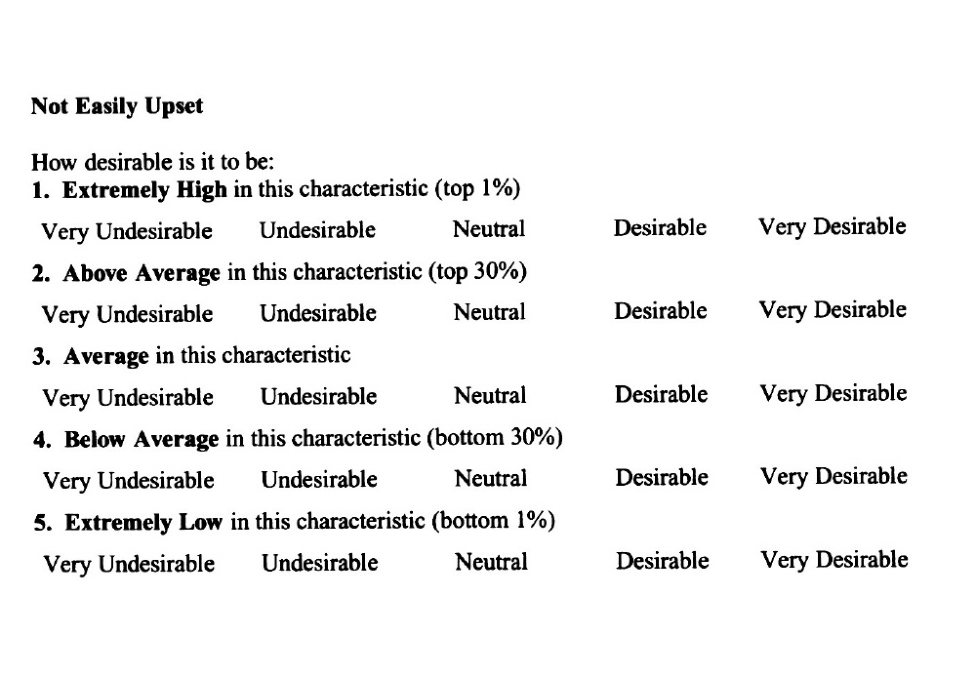
\includegraphics{KuncelTellegen_files/figure-latex/Figure1-1.pdf}
\caption{\label{fig:Figure1}Kuncel and Tellegen (2009) protocol for determining socially desirable saturation at the item response level.}
\end{figure}

Although there is both theoretical and empirical support for Kuncel and Tellegen (2009)'s procedure, it also quite substantially more time- and (we propose) effort-intensive than is the traditional item-rating approach (Edwards, 1953, 1957b). As technically specified, the traditional Edwards procedure requires one evaluation per item (albeit that evaluation is made across nine gradiated social desirability strata). The contemporary ``Kuncel and Tellegen'' procedure requires (in the case of 5-point Likert-type indicators) five evaluations across five levels of desirability per item. In addition to the greater \emph{number} of evaluations required in the contemporary approach, we propose that the contemporary approach is also likely more cognitively demanding due to shifting objects of reference (the referent of appraisal shifts across ratings - top 1\%, top 30\%, etc.).

Given the greater time and resource commitments required of the contemporary approach relative to the traditional, we aim to gauge to what extent these two approaches in fact capture similar versus unique pieces of information. The goal of the present investigation is therefore to directly compare these two methodologies with an ``additional information'' orientation - that is, is the new approach truly unique, or rather does it at least with some indicators convey somewhat redundant information as the classic, less cognitively taxing and more time-efficient approach?

\begin{quote}
\emph{Research Question 1}: Do the contemporary and traditional rating procedures capture redundant or unique information regarding social desirability saturation?
\end{quote}

\begin{quote}
\emph{Research Question 2}: Is the contemporary procedure more cognitively taxing than the traditional procedure? \(\leftarrow\) \textbf{Reword after finanlize analyses - didn't collect response latencies from the Edwards form}
\end{quote}

\hypertarget{study-1}{%
\section{Study 1}\label{study-1}}

\hypertarget{methods}{%
\section{Methods}\label{methods}}

\hypertarget{participants}{%
\subsection{Participants}\label{participants}}

Seventy-six undergraduate students made ratings of \emph{either} item social desirability (\emph{n} = 14, Edwards, 1957b), or levels of desirability associated with different trait levels (\emph{n} = 62, e.g., Kuncel \& Tellegen, 2009).

\hypertarget{materials}{%
\subsection{Materials}\label{materials}}

The IPIP-NEO is a 300-item personality measure intended to assess the Big Five personality dimensions: Conscientiousness, Agreeableness, Extraversion, Openness to Experience, and Neuroticism (Johnson, 2005). For the purposes of the current investigation, we did not collect typical responses to these 300 indicators, but were rather interested in the evaluative content of the items (or, alternatively, the evaluative content associated with differential standing along the construct implied by the item response options).

\hypertarget{procedure}{%
\subsection{Procedure}\label{procedure}}

All ratings were made via paper and pencil in an experimental laboratory. The Edwards (1957b) ratings were made along Edwards' originally specified 9-point scale ranging from Extremely Undesirable to Extremely Desirable. Because we investigated a fairly large instrument, we constructed 2 counterbalanced ``Edwards'' forms as an effort to limit potential fatigue effects across the rating process. The Kuncel and Tellegen (2009) ratings were collected from 60 different item stems across 10 different counterbalancings. Each rater (regardless of task; item stem or response option rating) was therefore asked to perform 300 total ratings (either 1 evaluation per 300 items or 5 evaluations per 60 items).

\hypertarget{results}{%
\section{Results}\label{results}}

All analyses were performed in R version 4.3.1 (R Core Team, 2023). We leveraged three different approaches comparing findings across the two item rating procedures. First, we fit linear regressions to all ``Kuncel \& Tellegen'' functions (as explained below), extracting slope coefficients, then regressed Edwards' ratings on these slopes across items. Secondly, we collected visual estimates of the monotonicity and linearity of these functions, and used these estimates to help inform ranges of Edwards values along which nonlinear item functions tend to be more prominent (e.g., how many ``inverted U-shaped'' functions were noted in items characterized by Edwards' system as \emph{extremely undesirable}, \emph{undesirable}, \emph{average}, \emph{desirable}, and \emph{extremely desirable}). Lastly, we conducted 300 hierarchical polynomial regressions to capture ``U'' or ``inverted-U'' functional forms, and tallied how many items were incrementally characterized by a quadratic (``above and beyond'' the linear) equation.

All three approaches focused on the \emph{functional form} of ``Kuncel \& Tellegen'' ratings. These ``functions'' reflect progression across Kuncel \& Tellegen frames of reference (ranging from someone who is ``Extremely High in the characteristic'' to someone who is ``Extremely Low in the characteristic'', again see Figure \ref{fig:Figure1} for exposition). The height of the function at each of these 5 levels is determined by the average desirability value at each of the focal item's 5 response categories.

\hypertarget{approach-1-functional-slope}{%
\subsubsection{Approach \#1: Functional Slope}\label{approach-1-functional-slope}}

One reasonable manifestation of redundancy across the two procedures would be greater incidences of linearity with extremely desirable (and undesirable) items. For the first investigative approach, we therefore probed for associations between ``Edwards''' item ratings and \emph{regression slope} of ``Kuncel \& Tellegen'' function.

We first fit 300 individual regressions retaining the five different rated trait locations as a predictor (e.g., Kuncel and Tellegen (2009)'s ``bottom 1\%'', ``bottom 30\%'', ``Average'', ``top 30\%'', and ``top 1\%'' - these were treated as a scaled continuum {[}values of 1, 2, 3, 4, and 5{]}) and averaged response desirability rating as the criterion. Within each of the 300 regressions, the expectation was that slope magnitude and valence would parallel the classic Edwards ratings of the same items. For example, the expectation was that an item such as ``Believe that others have good intentions'' would realize negative slope estimates, ``Enjoy wild flights of fancy'' would exhibit a flat slope, and ``Get irritated easily'' would return a moderately positive slope. Across all 300 items, the relationship was strong (\(R^2 = .58\), \(F_{(1,298)} = 412.26\), \emph{p} \textless{} .05), suggesting some level of similarity across procedures.

Figure \ref{fig:Figure2} presents ``Kuncel \& Tellegen'' functional forms for 25 items. These items were randomly selected from within five categorized Edwards arrays\footnote{Note that these plotted functions progress along only 5 actual x-axis values. The ``connected dots'' do not imply continuous x-axis values but are presented to facilitate observation of linear, monotonic, or non-monotonic functional patterns (e.g., Kuncel \& Tellegen, 2009).}, and the figure \emph{rows} reflect these strata. Note that the functions (even if somewhat non-monotonic - see, for example, ``Seldom Daydream'' in Figure \ref{fig:Figure2}) tend to exhibit ``steeper slope'' with Edwards' highly desirable or undesirable items, and are ``flatter'' with Edwards' moderate items - this first exploration merely confirms a general pattern such that more extreme ``Edwards'' items tend to have steeper ``Kuncel \& Tellegen'' functions, but is not sensitive to functional form (e.g., this is insensitive to ``monotonicity'').

\hypertarget{approach-2-functional-form-visual}{%
\subsubsection{Approach \#2: Functional form (Visual)}\label{approach-2-functional-form-visual}}

Next, the Figure \ref{fig:Figure2} plots for all 300 items were presented to judges who rated the visual functions along dimensions of ``on the whole, this looks like a straight line'' with possible ratings ranging from (1 = not at all, to 5 = definitely), and how much the ``line rises and falls'' from (1 = not at all, to 5 = a lot). These estimates were added to the first approach (defining each Edwards/Kuncel and Tellegen convergence with ratings of both functional linearity and monotonicity) and the result is presented in Figure \ref{fig:lastone}. Careful inspection of the Figure \ref{fig:lastone} plot again highlights the location of non-monotonic and nonlinear Kuncel and Tellegen functions - predominantly at moderate (around neutral) Edwards rating locations. {[}NOTE - LOOKS LIKE WE MAY NEED TO REDO THESE ESTIMATES; THERE ARE 96 ``NOT AT ALL LOOKS LIKE A STRAIGHT LINE'' and 130 ``NOT AT ALL RISES AND FALLS''; ALTERNATIVELY GET MORE CREATIVE WITH RESIDUALS ANALYSES (ON DESKTOP){]}

\begin{quote}
NOTE. Maybe do something with residuals to replace current subjective rating graph - lm object is named, ``try'' 8/12/23
\end{quote}

\hypertarget{approach-3-functional-form-empirical}{%
\subsubsection{Approach \#3: Functional form (Empirical)}\label{approach-3-functional-form-empirical}}

Our third approach leveraged hierarchical polynomial regressions, with our index of interest being the change in \(R^2\) at the second step, when the polynomial terms were specified. Most items (\(n_k\) = 203) had a very low change in \(R^2\) (see Table 1 ??? for a summary of these results and a specification of our definition of ``low'' or ``very low''). Beyond our subjective categorization, \(F\)-tests indicated that 92.31\% of item ratings were \emph{not} significantly predicted when specifying the quadratic term, and only 7.69\% were. \textbf{FIND THESE ANALYSES (7/29/23)}

\hypertarget{results-summary}{%
\subsection{Results Summary}\label{results-summary}}

Across approaches, results tended to converge on similar conclusions. The preponderance of our results first suggest that, in general (at least with our focal 300-item measure), linear relationships with social desirability (across response options) may be commonplace and in fact fairly well represent the plurarity of assessment item functions. Additionally, similar information seems to be available through both the traditional and contemporary measurement approaches. Although non-monotonic functions do exist, they are predominantly associated with moderately rated Edwards items. Cursory review of our randomly sampled 25 items (Figure \ref{fig:Figure2}) would agree with this conclusion.\footnote{A full list of all 300 item functions are available in this paper's online resources.} It is quite plausible that ``U'' or ``inverted U'' shaped functions, when they occur, are reflective of some ambiguous or contextually primed desirability, and that this ambiguity or contextual moderation results in ``middle ground'' evaluation via the Edwards method.

\hypertarget{study-two}{%
\section{Study Two}\label{study-two}}

\begin{quote}
put in some references regarding response latencies
\end{quote}

One of our observations across the two item rating procedures has been that the Kuncel and Tellegen (2009) approach appears to be more cognitively taxing for raters than does the Edwards (1953). Study Two therefore collected ratings via computer, with response latencies recorded as well as direct self-reported estimates of difficulty. The same indicators were retained for Study Two.

\hypertarget{procedure-1}{%
\subsection{Procedure}\label{procedure-1}}

The Study One items were administered via Qualtrics (2014). Participants were administered directions for each condition: 1) Edwards rating, 2) Kuncel \& Tellegen rating, and 3) modified Kuncel \& Tellegen rating. This third condition was included as a possible compromise to the \emph{anticipated} cognitive difficulty associated with the Kuncel \& Tellegen procedure. Here, we ask participants to focus on only one of the Kuncel \& Tellegen ``levels'' (e.g., across items, the rating category is held constant). We coded items for length and presence of a ``negative'' qualifier (e.g., I would never lie). Anecdotally, the presence of a negative element within an item stem contributed to difficulty for raters.

In addition to actual ratings, we also recorded latencies, which we interpret as indirect assessments of difficulty.

Because of the tedium and cognitive complexity of the requested task, we computed consecutive non-differentiating responses as well as intra-individual response variability estimates (see, for example, Dunn et al., 2018; Marjanovic et al., 2015) via the \emph{careless} R package (Yentes \& Wilhelm, 2023) in R version 4.3.1 (R Core Team, 2023).

Table to add: ICC's for each condition

Focus on response latencies (Edwards ratings vs.~Kuncel \& Tellegen vs.~revised Kuncel \& Tellegen (split by rated category). Indices here are: 1) response latencies, 2) inter-rater agreement/reliability \footnote{NOTE TO SELVES - WHEN WE DO THE SECOND PART (RESPONSE LATENCIES), MAKE SURE TO CODE NEGATIVELY-WORDED STEMS (THESE SEEM ESPECIALLY DIFFICULT TO RATE USING THE KUNCEL \& TELLEGEN PROCEDURE)}

\hypertarget{results-1}{%
\section{Results}\label{results-1}}

\begin{verbatim}
## Warning: Using `size` aesthetic for lines was deprecated in ggplot2 3.4.0.
## i Please use `linewidth` instead.
## This warning is displayed once every 8 hours.
## Call `lifecycle::last_lifecycle_warnings()` to see where this warning was
## generated.
\end{verbatim}

\begin{figure}
\centering
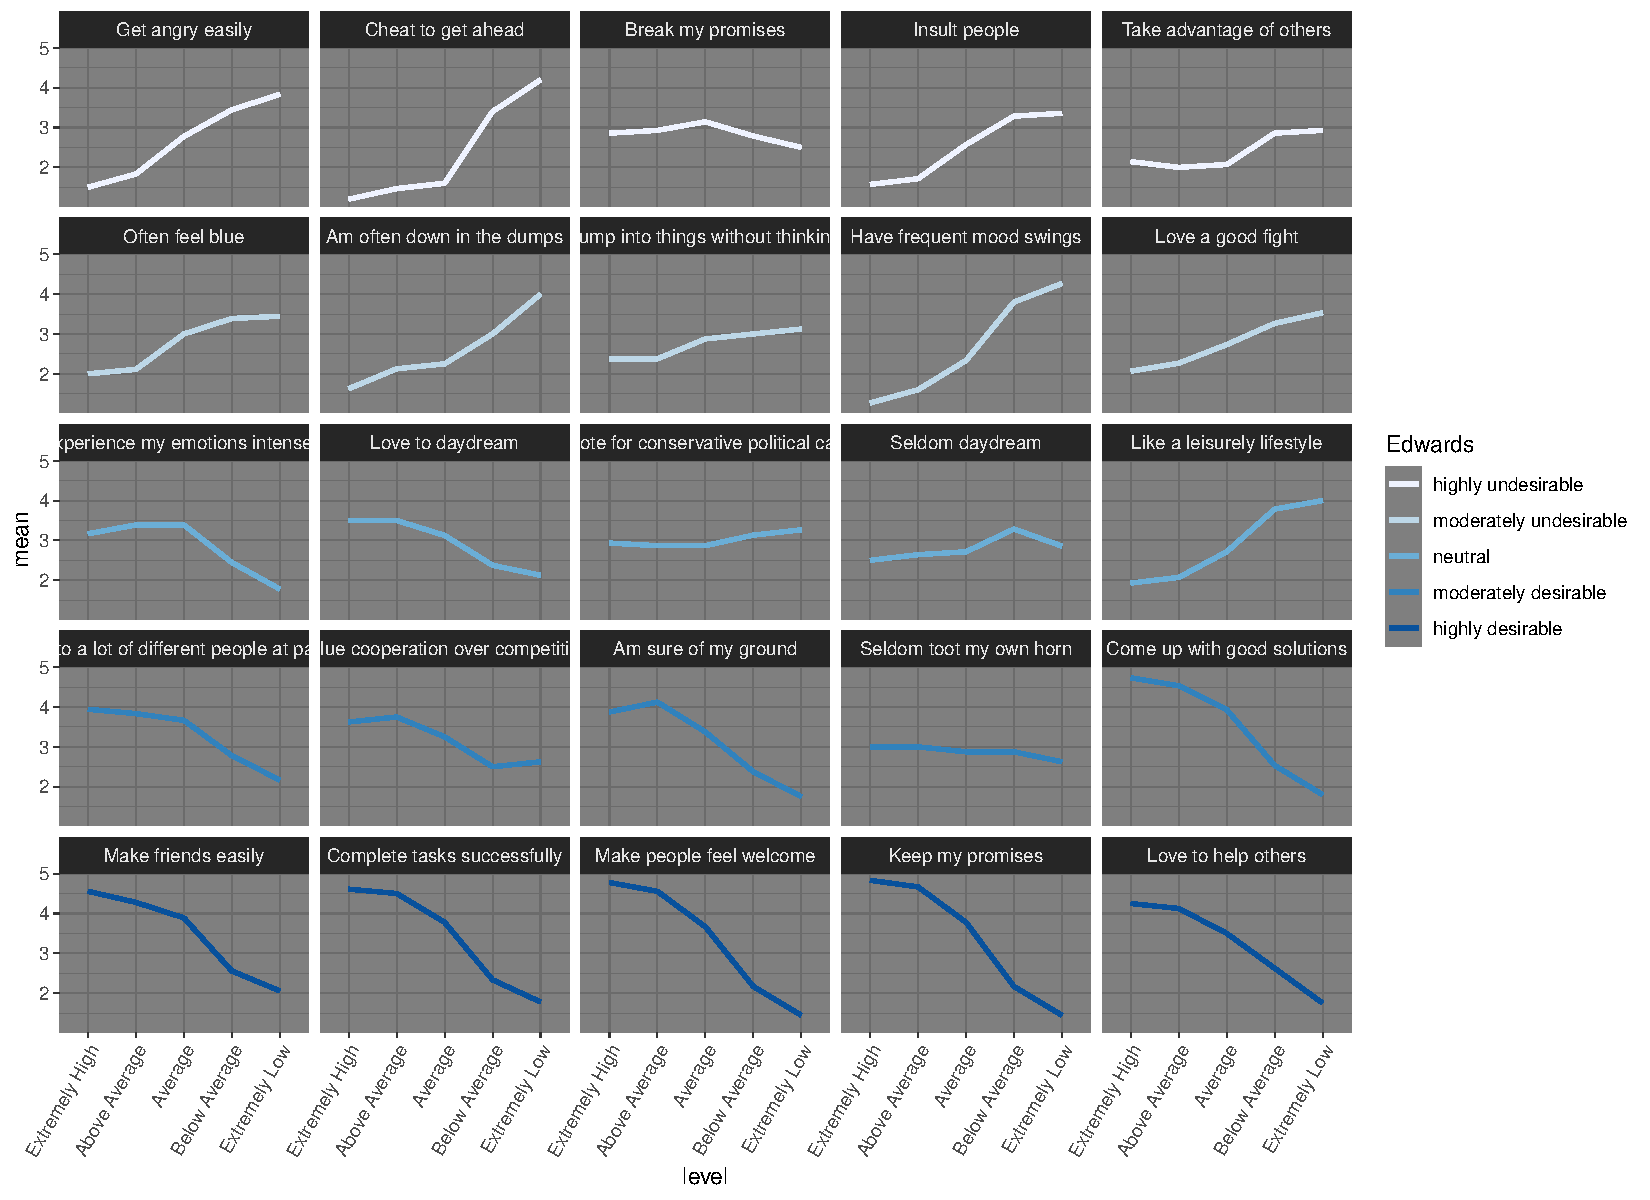
\includegraphics{KuncelTellegen_files/figure-latex/Figure2-1.pdf}
\caption{\label{fig:Figure2}Kuncel \& Tellegen (2009) patterns across Edwards (1953) scale values.}
\end{figure}

\begin{verbatim}
## Warning: Removed 46 rows containing missing values (`geom_point()`).
\end{verbatim}

\begin{figure}
\centering
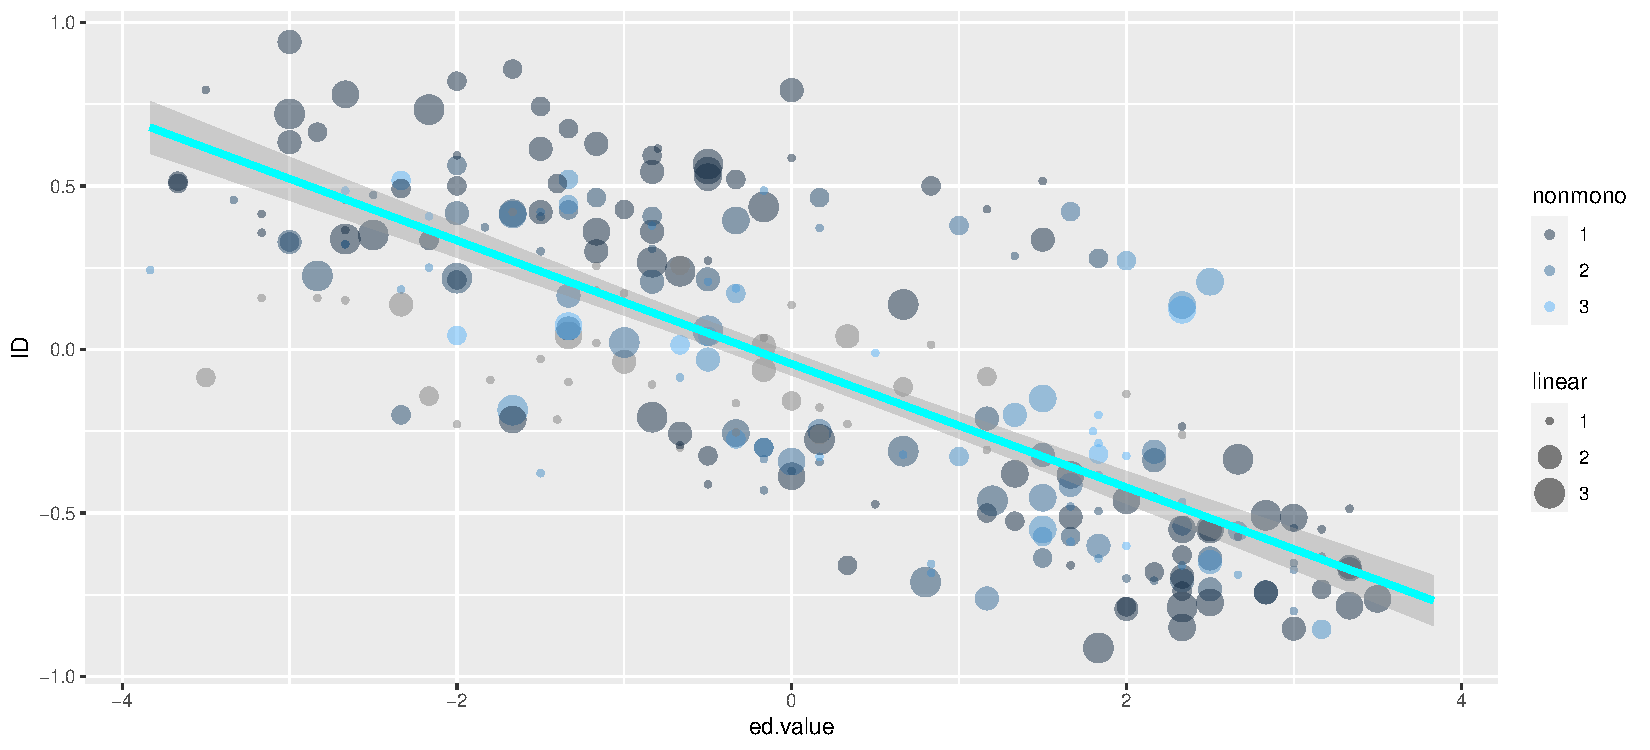
\includegraphics{KuncelTellegen_files/figure-latex/lastone-1.pdf}
\caption{\label{fig:lastone}Response Category and Mean Rating slope across Edwards' scale values (individual scatterpoints represent items).}
\end{figure}

The intercept was -3.08 \textless- just testing.

Looking at the function plots for the 15 Study 2 items (but retaining Study 1 data to create the functions), a better description (than linear, monotonic, etc) may be: 1) bipolar (good to be on one side, bad to be on the other), 2) moderate (best to be exactly in the middle), and 3) unipolar (good/bad to be on one side, ambivalent regarding other).

\hypertarget{discussion}{%
\section{Discussion}\label{discussion}}

The plurality of findings do support similar information being conveyed through both approaches. Figure 1 captures \emph{some} of this, as functional slopes (even if somewhat nonmonotonic - see, for example, ``Seldom Daydream'' in Figure 1) tend to be more extreme with Edwards' highly desirable or undesirable items, and more flat with Edwards' moderate items.\footnote{These items were randomly sampled from within Edwards-rating strata. Visuals of all items' functional forms are available from the authors upon request.} Table 1 presents the frequency with which researcher-implicated functional shapes (linear {[}positive{]}, linear {[}negative{]}, nonmonotonic {[}U{]}, and nonmonotonic {[}inverted U{]}) were noted within ``Edwardian'' strata, demonstrating that although the nonmonotonic functions do exist, they are predominantly associated with moderate Edwards items (e.g., yes these functions do occur but perhaps the ambivalence is also associated with aggregate moderation). Figure 2 presents the relationship between: 1) the functional slope relating an item response's rated level of desirability and the ``location'' of the rating, and 2) Edwards' item stem rating (on the y-axis). This strong relationship (\emph{R}\^{}2 = .67, \emph{p} \textless{} .05) suggests some level of similarity across procedures.

Undoubtedly, the Kuncel and Tellegen (2009) procedure conveys information not contained in the classic Edwards (1957b) approach. The purpose of this investigation, however, was to document overlap between the two procedures. While it is clear nonmonotonic functions do exist for some indicators across scaled ``trait levels,'' the vast majority of such circumstances are located within a range what the Edwards (1957b) procedure labels as merely moderately desirable or undesirable. There is surely additional information contained within these items, but the current investigation suggests that perhaps the more cognitively taxing and time-intensive procedure should be retained only for the items first identified by the cognitively-easier and less time-consuming Edwards (1957b) method. Our recommendation is to therefore retain both procedures, utilizing the cognitively easier and less time-consuming procedure as an initial evaluation and following-up with moderately desirable items to probe for more complex relationships.

Certainly the Kuncel and Tellegen (2009) procedure conveys information not contained in the classic Edwards (1957b) approach. The purpose of this investigation, however, was to document overlap between the two procedures. Clearly nonmonotonic functions do exist for some indicators across scaled ``trait levels''. However, the vast majority of such circumstances are located within what the Edwards (1957b) procedure labels as ``moderately desirable''. There is certainly additional information contained within these items, but the current investigation suggests that perhaps the more cognitively taxing and time-intensive procedure be retained for only those items first identified by the cognitively-easier and less time consuming Edwards (1957b) method as ``moderately desirable''.

\hypertarget{limitations}{%
\subsection{Limitations}\label{limitations}}

Our task was likely too long - in retrospect a shorter measure should have been pursued.

\begin{quote}
\textbf{Redundant with previous paragraph} \(\rightarrow\) In order to capture the extremity of function across Kuncel and Tellegen (2009) values, several regressions were fit using the average (across respondents) rating as a predictor (e.g., Kuncel and Tellegen (2009)`s ``Lower 1\%'', ``Lower 30\%'', ``Median'', ``Upper 30\%'', and ``Upper 1\%'' were treated as a scaled continuum) and average Edwards' desirability rating as the criterion. Slopes were retained for each function, with the expectation that slope magnitude and valence would parallel the classic Edwards ratings.
\end{quote}

\hypertarget{references}{%
\section{References}\label{references}}

\begingroup
\setlength{\parindent}{-0.5in}
\setlength{\leftskip}{0.5in}

\hypertarget{refs}{}
\begin{CSLReferences}{1}{0}
\leavevmode\vadjust pre{\hypertarget{ref-alicke_self-enhancement_2009}{}}%
Alicke, M. D., \& Sedikides, C. (2009). Self-enhancement and self-protection: What they are and what they do. \emph{European Review of Social Psychology}, \emph{20}(1), 1--48.

\leavevmode\vadjust pre{\hypertarget{ref-alicke_handbook_2011}{}}%
Alicke, M. D., \& Sedikides, C. (2011). \emph{Handbook of self-enhancement and self-protection}. Guilford Press.

\leavevmode\vadjust pre{\hypertarget{ref-R-papaja}{}}%
Aust, F., \& Barth, M. (2023). \emph{Papaja: Prepare american psychological association journal articles with r markdown}. \url{https://github.com/crsh/papaja}

\leavevmode\vadjust pre{\hypertarget{ref-barrick_what_2009}{}}%
Barrick, M. R., Shaffer, J. A., \& DeGrassi, S. W. (2009). What you see may not be what you get: Relationships among self-presentation tactics and ratings of interview and job performance. \emph{Journal of Applied Psychology}, \emph{94}(6), 1394.

\leavevmode\vadjust pre{\hypertarget{ref-birkeland_meta-analytic_2006}{}}%
Birkeland, S. A., Manson, T. M., Kisamore, J. L., Brannick, M. T., \& Smith, M. A. (2006). A meta-analytic investigation of job applicant faking on personality measures. \emph{International Journal of Selection and Assessment}, \emph{14}(4), 317--335.

\leavevmode\vadjust pre{\hypertarget{ref-crowne_new_1960}{}}%
Crowne, D. P., \& Marlowe, D. (1960). A new scale of social desirability independent of psychopathology. \emph{Journal of Consulting Psychology}, \emph{24}(4), 349.

\leavevmode\vadjust pre{\hypertarget{ref-cui2022distinguishing}{}}%
Cui, T., Kam, C. C. S., Cheng, E. H., \& Ho, M. Y. (2022). Distinguishing between trait desirability and item desirability in predicting item scores: Is informant evaluation of personality free from social desirability? \emph{Personality and Individual Differences}, \emph{196}, 111708.

\leavevmode\vadjust pre{\hypertarget{ref-dauenheimer_self-enhancement_2002}{}}%
Dauenheimer, D. G., Stahlberg, D., Spreemann, S., \& Sedikides, C. (2002). Self-enhancement, self-verification, or self-assessment? The intricate role of trait modifiability in the self-evaluation process. \emph{Revue Internationale de Psychologie Sociale}.

\leavevmode\vadjust pre{\hypertarget{ref-dimoulas_patterns_1998}{}}%
Dimoulas, E., Wender, S., Keenan, J. P., Gallup, G., \& Goulet, N. (1998). Patterns of deception in human mating strategies. \emph{Journal of Psychology and the Behavioral Sciences}, \emph{12}, 39--42.

\leavevmode\vadjust pre{\hypertarget{ref-donovan_impact_2014}{}}%
Donovan, J. J., Dwight, S. A., \& Schneider, D. (2014). The impact of applicant faking on selection measures, hiring decisions, and employee performance. \emph{Journal of Business and Psychology}, \emph{29}(3), 479--493.

\leavevmode\vadjust pre{\hypertarget{ref-dunn_intra-individual_2018}{}}%
Dunn, A. M., Heggestad, E. D., Shanock, L. R., \& Theilgard, N. (2018). Intra-individual response variability as an indicator of insufficient effort responding: Comparison to other indicators and relationships with individual differences. \emph{Journal of Business and Psychology}, \emph{33}(1), 105--121.

\leavevmode\vadjust pre{\hypertarget{ref-edwards_relationship_1953}{}}%
Edwards, A. L. (1953). The relationship between the judged desirability of a trait and the probability that the trait will be endorsed. \emph{Journal of Applied Psychology}, \emph{37}(2), 90--93.

\leavevmode\vadjust pre{\hypertarget{ref-edwards_social_1957-4}{}}%
Edwards, A. L. (1957a). Social desirability and probability of endorsement of items in the interpersonal check list. \emph{The Journal of Abnormal and Social Psychology}, \emph{55}(3), 394--396.

\leavevmode\vadjust pre{\hypertarget{ref-edwards_social_1957}{}}%
Edwards, A. L. (1957b). \emph{The social desirability variable in personality assessment and research.}

\leavevmode\vadjust pre{\hypertarget{ref-kuncel_conceptual_2009}{}}%
Kuncel, N. R., \& Tellegen, A. (2009). A conceptual and empirical reexamination of the measurement of the social desirability of items: Implications for detecting desirable response style and scale development. \emph{Personnel Psychology}, \emph{62}(2), 201--228.

\leavevmode\vadjust pre{\hypertarget{ref-leising_vocabulary_2012}{}}%
Leising, D., Ostrovski, O., \& Borkenau, P. (2012). Vocabulary for describing disliked persons is more differentiated than vocabulary for describing liked persons. \emph{Journal of Research in Personality}, \emph{46}(4), 393--396.

\leavevmode\vadjust pre{\hypertarget{ref-leising_model_2015}{}}%
Leising, D., Scherbaum, S., Locke, K. D., \& Zimmermann, J. (2015). A model of {``substance''} and {``evaluation''} in person judgments. \emph{Journal of Research in Personality}, \emph{57}(1), 61--71.

\leavevmode\vadjust pre{\hypertarget{ref-leising2021correlations}{}}%
Leising, D., Vogel, D., Waller, V., \& Zimmermann, J. (2021). Correlations between person-descriptive items are predictable from the product of their mid-point-centered social desirability values. \emph{European Journal of Personality}, \emph{35}(5), 667--689.

\leavevmode\vadjust pre{\hypertarget{ref-levashina_model_2006}{}}%
Levashina, J., \& Campion, M. A. (2006). A model of faking likelihood in the employment interview. \emph{International Journal of Selection and Assessment}, \emph{14}(4), 299--316.

\leavevmode\vadjust pre{\hypertarget{ref-li_using_2006}{}}%
Li, A., \& Bagger, J. (2006). Using the {BIDR} to distinguish the effects of impression management and self-deception on the criterion validity of personality measures: A meta-analysis. \emph{International Journal of Selection and Assessment}, \emph{14}(2), 131--141.

\leavevmode\vadjust pre{\hypertarget{ref-marjanovic_inter-item_2015}{}}%
Marjanovic, Z., Holden, R., Struthers, W., Cribbie, R., \& Greenglass, E. (2015). The inter-item standard deviation ({ISD}): An index that discriminates between conscientious and random responders. \emph{Personality and Individual Differences}, \emph{84}, 79--83.

\leavevmode\vadjust pre{\hypertarget{ref-morgeson_reconsidering_2007}{}}%
Morgeson, F. P., Campion, M. A., Dipboye, R. L., Hollenbeck, J. R., Murphy, K., \& Schmitt, N. (2007). Reconsidering the use of personality tests in personnel selection contexts. \emph{Personnel Psychology}, \emph{60}(3), 683--729.

\leavevmode\vadjust pre{\hypertarget{ref-ones_role_1996}{}}%
Ones, D. S., Viswesvaran, C., \& Reiss, A. D. (1996). Role of social desirability in personality testing for personnel selection: The red herring. \emph{Journal of Applied Psychology}, \emph{81}(6), 660--679.

\leavevmode\vadjust pre{\hypertarget{ref-paulhus_balanced_1988}{}}%
Paulhus, D. L. (1988). Balanced inventory of desirable responding ({BIDR}). \emph{Acceptance and Commitment Therapy. Measures Package}, \emph{41}, 79586--79587.

\leavevmode\vadjust pre{\hypertarget{ref-qualtrics_qualtrics_2014}{}}%
Qualtrics, L. L. C. (2014). Qualtrics {[}software{]}. \emph{Utah, {USA}: Qualtrics}.

\leavevmode\vadjust pre{\hypertarget{ref-R-base}{}}%
R Core Team. (2023). \emph{R: A language and environment for statistical computing}. R Foundation for Statistical Computing. \url{https://www.R-project.org/}

\leavevmode\vadjust pre{\hypertarget{ref-sedikides_self-enhancement_2012}{}}%
Sedikides, C., \& Alicke, M. D. (2012). \emph{Self-enhancement and self-protection motives}. Oxford handbook of motivation, ed. R. Ryan. Oxford University Press.{[}{rWvH}{]}.

\leavevmode\vadjust pre{\hypertarget{ref-taylor_illusion_1988}{}}%
Taylor, S. E., \& Brown, J. D. (1988). Illusion and well-being: A social psychological perspective on mental health. \emph{Psychological Bulletin}, \emph{103}(2), 193.

\leavevmode\vadjust pre{\hypertarget{ref-viswesvaran_meta-analyses_1999}{}}%
Viswesvaran, C., \& Ones, D. S. (1999). Meta-analyses of fakability estimates: Implications for personality measurement. \emph{Educational and Psychological Measurement}, \emph{59}(2), 197--210.

\leavevmode\vadjust pre{\hypertarget{ref-weiss_looking_2006}{}}%
Weiss, B., \& Feldman, R. S. (2006). Looking good and lying to do it: Deception as an impression management strategy in job interviews. \emph{Journal of Applied Social Psychology}, \emph{36}(4), 1070--1086.

\leavevmode\vadjust pre{\hypertarget{ref-R-careless}{}}%
Yentes, R., \& Wilhelm, F. (2023). \emph{Careless: Procedures for computing indices of careless responding}. \url{https://github.com/ryentes/careless/}

\leavevmode\vadjust pre{\hypertarget{ref-ziegler_applicant_2011}{}}%
Ziegler, M. (2011). Applicant faking: A look into the black box. \emph{The Industrial and Organizational Psychologist}, \emph{49}(1), 29--36.

\end{CSLReferences}

\endgroup


\end{document}
